% TODO: remove figure[H] -> white space

\documentclass[12pt, a4paper]{memoir} % for a short document
\usepackage[french,english]{babel}

\usepackage [vscale=0.76,includehead]{geometry}                % See geometry.pdf to learn the layout options. There are lots.
%\geometry{a4paper}                   % ... or a4paper or a5paper or ...
%\geometry{landscape}                % Activate for for rotated page geometry
%\OnehalfSpacing
% \setSingleSpace{1.05}
%\usepackage[parfill]{parskip}    % Activate to begin paragraphs with an empty line rather than an indent
\usepackage{graphicx}
\usepackage{amsmath,amssymb}
\usepackage{amsfonts}
\usepackage{amsthm}
\usepackage{bbm}
\usepackage{fullpage}
\usepackage{mathptmx} % font = times
\usepackage{helvet} % font sf = helvetica
\usepackage[T1]{fontenc}
\usepackage[utf8]{inputenc}
\usepackage{relsize}
\usepackage{float}
\usepackage{accents}
\usepackage{caption}
\usepackage{subcaption}
\usepackage[all]{xy} % for diagrams

% Clickable links in the toc
\usepackage{hyperref}
\hypersetup{
    colorlinks,
    citecolor=black,
    filecolor=black,
    linkcolor=black,
    urlcolor=black
}

% Custom commands
\newcommand{\ocirc}[1]{\accentset{\circ}{#1}}
\newcommand{\R}{\mathbb{R}}
\newcommand{\partiald}[2]{\frac{\partial{#1}}{\partial{#2}}}
\newcommand{\indicator}[1]{\mathbbm{1}_{#1}}

% Custom options
% \setlength{\belowcaptionskip}{-5pt}

% Custom theorems
\newtheorem{definition}{Definition}
\newtheorem{proposition}{Proposition}
\newtheorem{lemma}{Lemma}
\newtheorem{theorem}{Theorem}

% Graphics path
\graphicspath{{img/}}

% Custom styles
\headstyles{komalike}
\nouppercaseheads
\chapterstyle{dash}
\makeevenhead{headings}{\sffamily\thepage}{}{\sffamily\leftmark}
\makeoddhead{headings}{\sffamily\rightmark}{}{\sffamily\thepage}
\makeoddfoot{plain}{}{}{} % Pages chapitre.
\makeheadrule{headings}{\textwidth}{\normalrulethickness}
%\renewcommand{\leftmark}{\thechapter ---}
\renewcommand{\chaptername}{\relax}
\renewcommand{\chaptitlefont}{ \sffamily\bfseries \LARGE}
\renewcommand{\chapnumfont}{ \sffamily\bfseries \LARGE}
\setsecnumdepth{subsection}

% Title page formatting -- do not change!
\pretitle{\HUGE\sffamily \bfseries\begin{center}}
\posttitle{\end{center}}
\preauthor{\LARGE  \sffamily \bfseries\begin{center}}
\postauthor{\par\end{center}}

\newcommand{\jury}[1]{%
\gdef\juryB{#1}}
\newcommand{\juryB}{}
\newcommand{\session}[1]{%
\gdef\sessionB{#1}}
\newcommand{\sessionB}{}
\newcommand{\option}[1]{%
\gdef\optionB{#1}}
\newcommand{\optionB}{}

\renewcommand{\maketitlehookd}{%
\vfill{}  \large\par\noindent
\begin{center}\juryB \bigskip\sessionB\end{center}
\vspace{-1.5cm}}
\renewcommand{\maketitlehooka}{%
\vspace{-1.5cm}\noindent\includegraphics[height=14ex]{logoINP.png}\hfill\raisebox{2ex}{\includegraphics[height=7ex]{logoUJF.jpg}}\\
\bigskip
\begin{center} \large
Master of Science in Informatics at Grenoble \\
Master Math\'ematiques Informatique - sp\'ecialit\'e Informatique \\
option \optionB  \end{center}\vfill}
% End of title page formatting

\option{$GVR$}
\title{Adaptive point cloud denoising}%\\\vspace{-1ex}\rule{10ex}{0.5pt} \\sub-title}
\author{Jocelyn MEYRON}
\date{ $<$Defense Date$>$} % Delete this line to display the current date
\jury{
Research project performed at GIPSA-lab \\\medskip
Under the supervision of:\\
ATTALI Dominique, GIPSA-lab\\
MÉRIGOT Quentin, Université Paris-Dauphine\\\medskip
Defended before a jury composed of:\\
Mr HÉTROY-WHEELER Franck\\
$[$Prof/Dr/Mrs/Mr$]$ $<$first-name last-name$>$\\
$[$Prof/Dr/Mrs/Mr$]$ $<$first-name last-name$>$\\
$[$Prof/Dr/Mrs/Mr$]$ $<$first-name last-name$>$\\
}
\session{$June$\hfill 2015}

\begin{document}

% Title page
\selectlanguage{english}
\frontmatter
\begin{titlingpage}
\maketitle
\end{titlingpage}
\setlength{\parskip}{-1pt plus 1pt}

% Abstract
\renewcommand{\abstracttextfont}{\normalfont}
\abstractintoc

% English
\begin{abstract}

% TODO
During this internship, we were interested in the denoising / smoothing of point
clouds sampled on an unknown surface. For doing that, we will use a mean
curvature flow approach: we will move the points while minimizing an energy, the
area of the underlying surface. So, we will need a way to approximate the area
of a surface by only knowing points sampled on it, we will use the volume of a
union of balls centered on the point cloud.  We will also be interested in
another kind of flow: an anisotropic one. The magnitude of the smoothing will be
more important in some directions dictated by the choice of the polyhedron. The
idea is to replace the union of balls by a union of convex polyhedra and do the
same work.

This report is divided as follows: firstly, we will give a detailed introduction
about point cloud smoothing: existing techniques and why using a mean curvature
flow can be interesting. Then, we will study the two dimensional case. We will
show that this technique can be used to simulate a discrete mean curvature flow
and so smooth point clouds. The technique can also be used to estimate the mean
curvature. Many examples will be studied. Furthermore, we will continue by
looking at the 3D case where we will study the volume of a union of convex
polyhedra. Several theoretical and practical issues will arise. We will explain
the choices that were mode to solve these issues. Finally, we will look at the
theory behind our approach.

\end{abstract}

\newpage
\abstractintoc
\renewcommand\abstractname{R\'{e}sum\'{e}}

% Français
\begin{abstract} \selectlanguage{french}

% TODO
Durant ce stage, nous nous sommes intéressés au débruitage / lissage de nuages
de points échantillonnés sur une surface inconnue. Pour faire cela, nous avons
utilisé une approche basée sur le flot de courbure moyenne: nous faisons évoluer
le nuage de points tout en minimisant une énergie, l'aire de la surface
sous-jacente. Donc, nous avons besoin d'un moyen pour approcher l'aire de la
surface en connaissant seulement des points échantillonnés sur celle-ci, nous
avons utilisé le volume de l'union des boules centrées sur le nuage de point.
Nous nous somme aussi intéressé à un autre genre de flot: un flot anisotropique.
La magnitude du flot sera plus importante dans certaines directions privilégiées
dictées par le choix du polyèdre. L'idée est de remplacer l'union des boules par
une union de polyèdres convexes et de faire le même type de travail.

Ce rapport est structuré de la manière suivante: tout d'abord, nous donnerons
une introduction détaillée sur les techniques existantes de lissage de nuages de
points et pourquoi il est intéressant d'avoir choisi une approche basée sur le
flot de courbure moyenne. Ensuite, nous étudierons le cas bidimensionnelle. Nous
montrerons que cette technique peut être utilisée pour simuler un flot de
courbure moyenne discret et donc de lisser des nuages de points. Cette technique
peut aussi être utilisée pour estimer la courbure moyenne. Beaucoup d'exemples
illustreront ces résultats. Par la suite, nous nous intéresserons au cas 3D pour
lequel nous étudierons le volume d'une union de polyèdres convexes. Nous serons
confrontés à des difficultés aussi bien théoriques que pratiques. Nous
expliquerons alors les choix qui ont été faits pour résoudre les problèmes
rencontrés. Enfin, nous nous intéresserons à la théorie utilisée derrière notre
approche.

\end{abstract}

\selectlanguage{english}

% vim: set spelllang=en :

\cleardoublepage

\tableofcontents* % the asterisk means that the table of contents itself isn't put into the ToC
\normalsize

\mainmatter
\SingleSpace

% Main matter
% partie logiciel:
% 2D

% 3D 1: intersection de demi-espaces -> associer plane + inter pour AD (lien avec AD), type de nombre
% 3D 2: inclusion-exclusion
% -> environ 3 pages + bouts de codes

% courbe de décroissance de l'aire en fonction du pas de temps
% exemples 2d lissage (carré)

\chapter{Introduction}

% TODO: contexte / state of the art
% TODO: annonce du plan

% {{{1 MOTIVATION
\section{Motivation}

The main motivation of this internship is to develop techniques for computing the
mean curvature flow on point clouds instead of surfaces.

This will have applications on denoising and smoothing of point clouds. Indeed,
the mean curvature flow is known for its smoothing properties (see
\cite{ciomaga2010level}).

For example, \ref{fig:mean-curvature-flow-ex} is an illustration of the mean
curvature flow on a noised surface (extracted from
\cite{clarenz2000anisotropic}).

\begin{figure}[h]
    \centering
    \includegraphics[scale=0.3]{img/mean-curvature-flow-rabbit}
    \caption{Mean curvature flow on a noised surface}
    \label{fig:mean-curvature-flow-ex}
\end{figure}

We will also tackle the problem of computing a curvature-related flow for
polyhedral norms (i.e. we will do the Minkowski sum of a point cloud with a
convex polyhedron). It will allow us to apply a denoising which will have some
privileged directions: the denoising / smoothing will have different effects in
these directions.

This will have applications, for example, in physics based simulations like
crystal growth simulation.  An other example would be when we build a 3D scan of
an object: we want to be able to smooth the point cloud while preserving details
(the signature of the author for example).

In the next section, we will describe in more details the continuous mean
curvature flow.

% TODO

% {{{1 MEAN CURVATURE FLOW
\section{Mean Curvature Flow}

Given a family of hypersurfaces $ S_t $ of $ \R^d $, we say that $ S_t $ is
evolving by mean curvature if it satisfies the following equation:

$$ \partiald{x}{t} = \vec{\kappa}(x) $$

Where $ \vec{\kappa}(x) $ is the mean curvature vector of $ S_t $ at $ x $ and
$ \partiald{x}{t} $ is the normal velocity.

Put in more simple words, it says that at each step we move each point of the
hypersurface $ S_t $ in the direction of the inward normal by an amount given by
the mean curvature.

Now, we will prove that the mean curvature flow belongs to a more general
category of geometric flows: the gradient flows. Given an energy $ f $, we say
that $ S $ evolves according to the gradient flow of $ f $ if we have:

$$ \partiald{x}{t} = \nabla f(x) $$

Indeed, the next proposition shows the relation between the mean curvature flow
and the area functional.

\begin{proposition}
    The mean curvature flow is the gradient flow of the area functional.
\end{proposition}

To prove this proposition, we will need some background on hypersurfaces.

First, the notion of the reach of an hypersurface: it is widely used in
computational geometry.
\begin{definition}
    The reach of a manifold $ M $ denoted by $ reach(M) $ is the largest $ r
    \geq 0 $ for which for any $ p \in M^r $, there exists a unique $ q \in M $
    such that $ q = p_M(p) $ where $ p_M $ is the projection on $ M $. $ p_M(x)
    $ is defined such that $ || x - p_M(x) || = d(x, M) $.
\end{definition}

For example, if we consider a circle in the plane of radius $ R $, then every
point in the plane has a unique projection on the circle except the center which
is at distance $ R $ of every point on the circle: there is no closest point.
Consequently, its reach is $ R $.

Another more general example is that any convex set has infinite reach. This is
because the projection on a closed convex set is uniquely defined.

The reach is also related to the Local Feature Size (LFS) defined in
\cite{amenta1999surface}: $ LFS(p) = d(p, \mathcal{M}) $ $ reach(M) =
\min\limits_{p \in M}~LFS(p) $ where $ \mathcal{M}  $ is the medial axis of $ M
$.

% TODO: exemples:
% reach < min (rayons de courbure) et dessin inégalité contraire fausse

Then, some facts about the curvature of embedded hypersurfaces:

\begin{proposition}
    For an hypersurface $ S \subseteq \R^d $, the map $ x \in S \rightarrow
    \vec{n}_S(x) $ where $ \vec{n}_S(x) $ is the normal vector of $ S $ at $ x $ is
    called the Gauss map while its derivative is called the shape operator.

    Then, we have that the shape operator is diagonalizable and its eigenvalues
    are the $ d-1 $ principal curvatures at $ x $: $ \kappa_1(x), \ldots,
    \kappa_{d-1}(x) $.

    We will also denote by $ \vec{\kappa}(x) $ the mean curvature vector at $ x
    $: $ \vec{\kappa}(x) = \sum_{i=1}^{d-1} \kappa_i(x) \vec{n}_S(x) $.
\end{proposition}

And finally, a change of variable result:

% TODO: reference
\begin{lemma}
    \label{lemma:diffeo}
    Given a smooth hypersurface $ S $, and a function $ f : S \times [0, r] \to \R^d $
    defined by $ f(x, t) = x + t \phi(x) \vec{n}_S(x) $ where $ \phi : \R^d \to
    \R^d $ is a smooth vector field then $ f $ is a diffeomorphism for $ r < reach(S) $.

    If we decompose this substitution on $ T_p(S) \times [-r, r] $, where $ T_p(S)
    $ is the tangent space of $ S $ at $ p $, we get: $ D \phi = id + r D
    \vec{n_S}(q) $.  So, its Jacobian is given by: $ J_f(x) = \det(id + t \phi(x) D
    \vec{n}_S (x)) $.

    Using the previous proposition, we get:
    $$ J_f(x) = \prod_{i=1}^{d-1} (1 + t \phi(x) \kappa_i(x)) $$
\end{lemma}

We will denote by $ Vol^d(S) $ the $d$-dimensional volume of an object $ S
$.

Then, we can tackle the proof:

\begin{proof}
    We parametrize the evolving surface $ S_t $ by $ S_t = \{ x + t \phi(x)
    \vec{n}(x), x \in S_0\} $ where $ \phi : \R^d \rightarrow \R^d $ is a smooth
    vector field. We denote by $ A = Vol^{d-1} $ the area functional.
    Then, we have, using the lemma \ref{lemma:diffeo}:
    \begin{align*}
        Vol^{d-1}(S_t) &= \int_{S_t} 1 dx = \int_{S_0} J_{\phi}(x) dx \\
        &= \int_{S_0} \prod_{i=1}^{d-1} (1 + t \phi(x) \kappa_i(x)) \\
        &= \int_{S_0} 1dx + t \int_{S_0} \phi(x) \vec{\kappa}(x) dx + O(t^2)
    \end{align*}

    So:
    $$ \lim\limits_{t \to 0} \frac{A(S_t) - A(S_0)}{t}= \int_{S_0}
    \phi(x) \vec{\kappa}(x) dx $$

    This equation tells us exactly that the variation of the area functional is
    linked to the mean curvature.
\end{proof}

This proposition will be at the basis of our work. We will replace "hypersurface"
with "point cloud sampled on an hypersurface" and try to approximate the area of
the hypersurface by something which can be computed using only the point cloud.

% {{{1 DISCRETIZATION OF THE AREA
\section{Discretization of the area}

In this section, we will try to compute an approximation of the area of an
hypersurface with only knowing points sampled on it.

First, we will introduce the $r$-offset of a point cloud:

\begin{definition}
    For $ r > 0 $ and a point cloud $ P $, we define the $r$-offset of $ P $
    denoted by $ P^r $ by:
    $$ P^r = \bigcup_{p \in P} B(p, r)$$
\end{definition}

It can also be seen as the Minkowski sum of $ P $ and the euclidean ball $ B(0,
r) $.

\begin{definition}
    For any sets $ A $ and $ B $ of a vector space, we define the Minkowski sum
    of $ A $ and $ B $ denoted by $ A \oplus B $:
    $$ A \oplus B = \{ a + b, a \in A, b \in B \} $$
\end{definition}

Then, we will define a similar notion for hypersurfaces called the tubular
neighbourhood:

\begin{definition}
    For any $ r > 0 $, the tubular neighbourhood of an hypersurface $ S $
    denoted by $ S^r $ is the set of all points $ x \in \R^d $ such that there
    exists $ y \in S $ and $ d(x, y) \leq r $.
\end{definition}

Using these notions, we can relate the area of an hypersurface to the volume of
its tubular neighbourhood using a variant of the tube formula \cite{weyl1939volume}.

\begin{proposition}
    \label{prop:comp-offset-area}
    If $ S $ is a smooth hypersurface whose reach is positive and $ reach(S) > r
    > 0 $, then: $$ Vol^{d-1}(S) = \frac{Vol^d(S^r)}{2r} + O(r^2) $$

    The constants in the reset of the development only depend on the curvature
    of $ S $.
\end{proposition}

\begin{proof}
    We have: $ Vol^d(S^r) = \int_{S^r} 1 dx $.

    Now, we will do the following change of variable: $ \phi : S \times [-r, r]
\rightarrow S^r $ where $ \phi(x, t) = x + t \vec{n}_K(x) $.

    Using this substitution and the lemma \ref{lemma:diffeo} with $ \phi = 1 $:

    \begin{align*}
        Vol^d(S^r) &= \int_S \int_{-r}^r J_{\phi}(p) dt dp \\
        &= \int_S \int_{-r}^r \prod_{i=1}^{d-1} (1 + t \kappa_i(p)) dt dp \\
        &= \int_S \int_{-r}^r \left( 1 + \sum_{k=1}^{d-1} t^k \sum_{i_1 < \ldots
                < i_k} \kappa_{i_1}(p) \ldots \kappa_{i_k}(p) \right) dt dp \\
        &= 2r \int_S 1 dp + \int_K \int_{-r}^r \sum_{k=1}^{d-1} t^k \sum_{i_1 < \ldots < i_k} \kappa_{i_1}(p) \ldots \kappa_{i_k}(p) dt dp \\
        &= 2r Vol^{d-1}(S) + O(r^2)
    \end{align*}

    So: $ \frac{Vol^d(S^r)}{2r} = Vol^{d-1}(S) + O(r^2) $.
\end{proof}

This proposition is related to the Minkowski content. It is used to measure the
area of the boundary of a set: the $ d-1 $ dimensional volume in dimension $ d
$.

It is defined as follows:
$$ \lim\limits_{\epsilon \to 0} \frac{\mu(S^{\epsilon}) - \mu(S)}{\epsilon} $$

This is exactly what we computed: a Taylor expansion of $ Vol^d(S^r) $.

Next, we want to approximate $ Vol^d(S^r) $ by $ Vol^d(P^r) $ where $ P \subset
S $ is a point cloud. We will need a formalization of the notion of sampling:

\begin{definition}
    A set of points $ p_i $ is said to be an $\epsilon$-sampling of a manifold $
    M $ if the set of the balls  $ B(p_i, \epsilon) $ verifies: $ M \subseteq
    \bigcup_i B(p_i, \epsilon) $ (see \cite{amenta1999surface}).
\end{definition}

The following proposition bounds the error of this approximation:

\begin{proposition}
    \label{prop:comp-vol-offsets}
    For an hypersurface $ S $ with positive reach and an $\epsilon$-sampling $ P
    \subseteq S $, we have:
    $$ 0 \leq Vol^d(S^r) - Vol^d(P^r) \leq \frac{\epsilon^2}{r} Vol^{d-1}(S) +
    O(\frac{\epsilon^4}{r^2}) $$
\end{proposition}

\begin{proof}
    Since $ P \subseteq S $, then $ Vol^d(S^r) \leq Vol^d(P^r) $.

    Then, we parametrize $ P^r $ by $ f : S \rightarrow P^r $ where $ f(x) = x +
    r(x) \vec{n}_S(x) $ for $ r(x) \in [0, r] $ (see
    \ref{fig:offset-parametrization}).

    \begin{figure}[h]
        \centering
        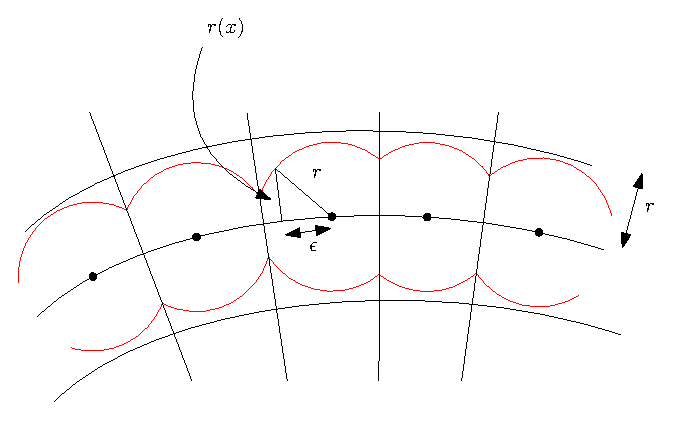
\includegraphics[scale=0.8]{offset-parametrization}
        \caption{Parametrization of the offset (in red)}
        \label{fig:offset-parametrization}
    \end{figure}

    We have:
    \begin{align*}
        r(x)^2 + \epsilon^2 = r^2 \iff& (r - r(x)) (r + r(x)) = \epsilon^2 \\
        \iff& r - r(x) = \frac{\epsilon^2}{r + r(x)} \leq \frac{\epsilon^2}{r} \\
    \end{align*}

    Now, we will use the same formula as in the previous proofs:

    \begin{align*}
        Vol^d(S^r) - Vol^d(P^r) &= \int_{A^r \textbackslash P^r} 1 dp \\
        &= \int_S \int_{r(x)}^r \det(id + t D \vec{n}_S(p)) dt dp \\
        &= \int_S \int_{r(x)}^r \left( 1 + \sum_{k=1}^{d-1} t^k \sum_{i_1 < \ldots
                < i_k} \kappa_{i_1}(p) \ldots \kappa_{i_k}(p) \right) dt dp \\
        &= \int_S (r - r(x)) dp + O((r - r(x))^2) \\
        &\leq \frac{\epsilon^2}{r} Vol^{d-1}(S) + O(\frac{\epsilon^4}{r^2})
    \end{align*}
\end{proof}

Now, combining the previous propositions, we will show that we can approximate
the area of $ S $ by the volume of $ P^r $:

\begin{proposition}
    \label{prop:approx-volume-area}
    Given an hypersurface $ S $, an $\epsilon$-sampling of $ S $: $ P $, we
    have:
    $$ | \frac{Vol^d(P^r)}{2r} - Vol^{d-1}(S) | \leq \frac{\epsilon^2}{2r^2} +
    O(\frac{\epsilon^4}{r^3}) + O(r^2) $$

    So, when $ \frac{\epsilon}{r} $ and $ r $ vanish then $
    \frac{Vol^d(P^r)}{2r} $ converges towards the area of $ S $.
\end{proposition}

\begin{proof}
    We will use the propositions \ref{prop:comp-vol-offsets} and
    \ref{prop:comp-offset-area}.

    We have, using the triangle inequaltiy:
    \begin{align*}
        \left| \frac{Vol^d(P^r)}{2r} - Vol^{d-1}(S) \right| \leq& \left| \frac{Vol^d(P^r)}{2r} -
            \frac{Vol^d(S^r)}{2r} \right| + \left| \frac{Vol^d(S^r)}{2r} -
            Vol^{d-1}(S) \right| \\
        \leq& \frac{\epsilon^2}{2r^2} Vol^{d-1}(S) + O(\frac{\epsilon^4}{r^3}) + O(r^2) \\
    \end{align*}
\end{proof}

At this point, we have shown a way to approximate the area of an hypersurface
with a quantity proportional to the volume of the $r$-offset of a point cloud
sampled on the surface.
Now, we want to study the gradient of this newly computed quantity.

% TODO

% {{{1 CONVERGENCE OF THE GRADIENT
\section{Convergence of the gradient}

In this section, we will derive formulae for the gradients of the volume of
union of balls in $ \R^d $.

The next proposition gives the gradient of the volume of union of balls :
\begin{proposition}
    Given an hypersurface $ S $ of $ \R^d $ and points sampled on it: $ (p_i) $.
    Then, if we denote by $ A $ the volume of the union of balls, we are
    interested in the variation of A by moving one point at a time.

    More precisely, we want to compute the following quantity: if we move the
    ith point by an amount $ \delta p_i $, what is the variation of $ A $:
    $$ \lim\limits_{\epsilon \to 0} \frac{A(p_1, \ldots, p_{i-1}, p_i + \epsilon
        \delta p_i, p_{i+1}, \ldots, p_N) - A(p_1, \ldots, p_N)}{\epsilon} $$

    We will denote this quantity $ \nabla_{p_i} A $. Then we have:
    \begin{equation}
        \label{eqn:gradient_area_2d}
        \nabla_{p_i} A = \int_{B} \frac{x - p_i}{||x - p_i||} dx
    \end{equation}
    where $ B = \partial B(p_i, r) \cap V(p_i, P) $ is the visible boundary of
    the ball.
\end{proposition}

Note that \cite{lachand2005minimizing} tackles the problem of minimizing a
functional over a convex body. For doing this, the authors compute the
derivatives of this functional: they use a similar technique we used for during
the proof of the previous proposition.

\begin{proof}

Let us say that we move the point $ p _i $ by a small quantity $ \delta p_i $,
let's study the variation of the area of $ \bigcup_i V(p_i, P) \cap B(p_i, r) $.

More formally, let's define $ A_{\epsilon} = A(V(p_i + \epsilon \delta p_i, P) \cap
B(p_i + \epsilon \delta p_i, r)) $, we want to compute the following limit:
$$ \lim\limits_{\epsilon \to 0} \frac{A_{\epsilon} - A_0}{\epsilon} $$

For computing this quantity, we will define the following sets:
\begin{itemize}
    \item $ B_1 = \{ x \in B, (x - p_i | \delta p_i) \geq 0\} $
    \item $ A_1^{\epsilon} = \bigcup_{x \in B_1} [x, x + \epsilon \delta p_i] $:
        "upper" gained area (see \ref{fig:demo-gradient} for a drawing of the
        situation in 2D)
    \item $ B_2 = \{ x \in B, (x - p_i | \delta p_i) \leq 0\} $
    \item $ A_2^{\epsilon} = \bigcup_{x \in B_2} [x, x + \epsilon \delta p_i] $:
        "lower" lost area.
\end{itemize}

\begin{figure}[h]
    \centering
    \includegraphics[scale=0.8]{2d/2d_proof_gradient_area_1}
    \caption{Situation for a ball $ B(p_i, r) $ in 2D}
    \label{fig:demo-gradient}
\end{figure}

Then, we have: $ A_\epsilon = A_0 + Vol(A_1^\epsilon) - Vol(A_2^\epsilon) +
O(\epsilon^2) $
% TODO

Now, we will approximate $ Vol(A_1^\epsilon) $ write that $ Vol(A_1^\epsilon) =
\int_{B_1} || x - z(x) || dx + o(||\delta p_i||) $. We do the same things for $
A_2^\epsilon $.

For any $ x \in B $, we define $ z(x) $ as the intersection of the half-line $ D
$ with the circle of center $ p_i + \epsilon \delta p_i $ of radius $ r $. We
also parametrize the half-line $ D $ by: $ x + t \frac{x - p_i}{||x - p_i||} $
where $ t \ge 0 $.

Let us find this intersection point by assuming that $ t $ is small
such that $ t^2 = t \delta p_i = o(||\delta p_i||^2) $.

We need to find $ D \cap C(p_i + \delta p_i, r) $. Let $ t \ge 0 $ then , we have :
\begin{equation}
    || x + t \frac{x - p_i}{||x - p_i||} - (p_i + \epsilon \delta p_i) ||^2 = r^2
    \tag{$\star$}
\end{equation}

If we expand this expression, we get:

\begin{align*}
    (\star) & \iff || x - (p_i + \epsilon \delta p_i) ||^2 + t^2 + 2t \left(
        \frac{x-p_i}{|| x - p_i||} | x - (p_i + \epsilon \delta p_i) \right) = r^2 \\
    & \iff || x - p_i || ^2 - 2 \epsilon (x - p_i | \delta p_i) + || \epsilon \delta p_i || ^2 + t^2 + 2t
    \left( \frac{x-p_i}{|| x - p_i||} | x - (p_i + \epsilon \delta p_i) \right) = r^2 \\
    & \iff -2 \epsilon (x - p_i | \delta p_i) + 2t || x - p_i|| + o(||\delta p_i||^2) = 0
    \text{ because } || x - p_i || = r \\
    & \iff t = t^{\star} = \epsilon \left( \frac{x - p_i}{||x - p_i||} | \delta p_i \right) +
    o(||\delta p_i||^2)
\end{align*}

Then, $ z(y) = x + t^{\star} \frac{x - p_i}{||x - p_i||} $ and $ || x - z(x) || =
t^{\star} $.

We deduce that :
$$ Vol(A_1^\epsilon) = \int_{B_1} \left[ \epsilon \left( \frac{x - p_i}{||x - p_i||} | \delta p_i \right) +
o(||\delta p_i||^2) \right] dx $$

And:

$$ Vol(A_1^\epsilon) - Vol(A_2^\epsilon) = \int_{B} \left[ \epsilon \left( \frac{x - p_i}{||x - p_i||} | \delta p_i \right)
+ o(||\delta p_i||^2) \right] dx $$

Finally, we have, by linearity:
$$ \nabla_{p_i} A = \int_{B} \frac{x - p_i}{||x - p_i||} dx $$

\end{proof}

Now, we will relate the previously computed gradients to the mean curvature
vector of an hypersurface.

If we suppose that we have a point cloud that is an $\epsilon$-sampling of a
smooth hypersurface $ S $, then the following proposition gives the link between
the gradient of volume of an offset of $ S $ and the mean curvature vector.

\begin{proposition}
    \label{prop:gradient-mean-curvature}
    Given an $\epsilon$-sampling $ P $ of a smooth ($ C^{\infty} $) hypersurface
    $ S $ and $ r \ge 0 $ such that: $ \epsilon \leq r \leq reach(M) $, then:
    $$ || \nabla_p A - \vec{\kappa}(p) || \leq TODO $$
    Consequently, when $ \epsilon $ and $ \frac{\epsilon}{r} $ vanish then
    $ \nabla_p A $ converges towards the mean curvature vector of $ S $ at $ p $.
    % TODO: ajouter dessins
\end{proposition}

To prove that, we will need two lemmas extracted from \cite{amenta1999surface}
which will tell us how the Voronoi cells look:
\begin{lemma}
    If $ S $ is an hypersurface, $ P $ an $\epsilon$-sampling of $ S $ and $ p
    \in P $, then:
    $$ V(p, P) \cap S \subseteq B\left(p, \frac{\epsilon}{1 - \epsilon}
        LFS(p)\right) $$
\end{lemma}

\begin{lemma}
    If $ S $ is an hypersurface, $ P $ an $\epsilon$-sampling of $ S $, $ p
    \in P $ and $ v \in V(p, P) $ such that $ d(p, v) \ge \nu LFS(p) $ for $ \nu
    > 0 $, then the angle at $ s $ between the vector $ v $ and the normal at
    the surface (oriented in the same direction) is at most $
    \arcsin(\frac{r}{\nu(1-r)}) + \arcsin(\frac{r}{(1-r)}) $.
\end{lemma}

These two lemmas tell us that the Voronoi cells are skinny (first lemma) and
long (second lemma).

\begin{proof}
We will first do two approximations on \ref{eqn:gradient_area_2d}:
\begin{enumerate}
    \item the first one is to suppose that the offset of $ S $ is close enough
        to the offset of $ P $. Using the computation done in
        \ref{prop:comp-vol-offsets}, we can say that the error made is in the
        order of $ O(\frac{\epsilon^2}{r}) $.
    \item the second one is that if the sampling is dense enough then we can
        replace $ p $ by the projection of $ x $ on $ S $: $ \forall p \in S,~x
        \in V(p, P),~p = p_S(x) + O(\epsilon) $, see figure
        \ref{fig:voronoi-cylinder}.  For this approximation to hold, it is
        necessary for the pointed out distance to be greater than $ \epsilon $
        i.e. $ r \gg \epsilon $ which means that $ \frac{\epsilon}{r} $ needs to
        vanish.
\end{enumerate}

\begin{figure}[h]
    \centering
    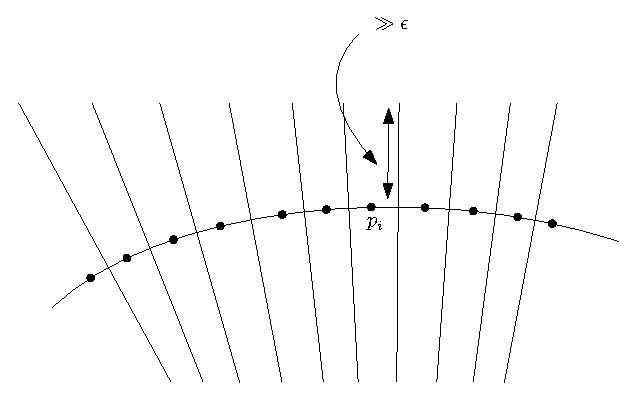
\includegraphics[scale=0.5]{img/voronoi-cylinder}
    \caption{Shape of the Voronoi cells of densely sampled points}
    \label{fig:voronoi-cylinder}
\end{figure}

Using these approximations, we get:
\begin{align*}
    \int_{\partial{P^r} \cap V(p, P)} (x - p) dx & \stackrel{(1)}{=} \int_{\partial{S^r} \cap V(p,
        P)} (x - p) dx + O(\epsilon^2) \\
    &\stackrel{(2)}{=} \int_{\partial{S^r} \cap V(p, P)} (x - p_S(x)) dx +
    O(\epsilon) \\
\end{align*}

Then, we will use the substitution $ q = p_S(x) \iff x = \phi(q) = q +
\vec{n_S}(q) $ where on the upper part of $ \partial{S^r} \cap V(p, P) $.

Using the lemma \ref{lemma:diffeo}, we have that $ \phi $ is a diffeomorphism
and that $ J_\phi(p) = (1 + \kappa_1(q)) (1 + \kappa_2(q)) $.

Using an analogous substitution on the lower part of $ \partial{S^r} \cap V(p,
P) $, we get : $ \det (D \phi) = (1 - \kappa_1(q)) (1 - \kappa_2(q)) $.

By summing the two, we obtain: $ 2 (\kappa_1(q) + \kappa_2(q)) $.

It follows that:
\begin{align*}
    \int_{\partial{S^r} \cap V(p, P)} (x - p_S(x)) dx &= \int_{S \cap V(p, P)}
    r \times \vec{n_S}(q) ( \det (id + r D \vec{n_S}(q)) - \det (id - r D
    \vec{n_S}(q)) ) dq \\
    &= 2r \int_{S \cap V(p, P)} (\kappa_1(q) + \kappa_2(q)) \vec{n_S}(q) dq \\
\end{align*}

% TODO: surface C infinie, constantes depéndent de la dérivée de la courbure
Finally, since we have supposed that $ S $ is $ C^{\infty} $ then, we can write:
$ \vec{n_S}(q) = \vec{n_S}(p) $, $ \kappa_1(q) = \kappa_1(p) $ and $ \kappa_2(q)
= \kappa_2(p) $. All the other terms depend on the derivatives of the curvature
which are negligible.

We deduce that:

$$ \nabla_p A = \partiald{A}{p} = 2r (\kappa_1(p) + \kappa_2(p)) \vec{n_S}(p)
\int_{S \cap V(p, P)} dq $$

So, using the mean curvature vector:

$$ \nabla_p A = 2r \vec{\kappa}(p) Vol(S \cap V(p, P)) $$

Which means:

$$ ||\nabla_p A - \vec{\kappa}(p) || \leq | 2r Vol(S \cap V(p, P)) - 1 |
\times|| \vec{\kappa}(p) ||$$

\end{proof}

We can summarize the situation with the following diagram:

\begin{displaymath}
    \xymatrix{A_r \ar[d]^{\nabla} \ar[r] & A \ar[d]^{\nabla} \\
        \nabla A_r \ar[r] & \nabla A }
\end{displaymath}

$ A_r $ represents the discretization of the area of an hypersurface: it
is $ \frac{Vol^d(P^r)}{2r} $ which converges towards the continuous area (see
proposition \ref{prop:approx-volume-area}). There is also a convergence property
for the gradients: the discretized gradient converges towards the continuous one
(see proposition \ref{prop:gradient-mean-curvature}).

In some sense, "discretization" and "gradient" commute: the gradient of the
discretization converges towards the continuous gradient.

% TODO

% {{{1 OTHER KINDS OF DISCRETIZATIONS
\section{Other kinds of discretizations}

% TODO: flot de l'aire du bord d'une surface = union de boules
In this work, we were also interested in other discretizations. Instead of
choosing the volume as the functional, we can also choose the area of the
boundary or corresponding weighted versions (i.e. the gradient of the volume
will be weighted by the corresponding volume of the intersection between the
Voronoi cell and a ball).

For the former case (area of the boundary), we have the following lemma:
\begin{lemma}
    If $ S $ is a smooth hypersurface whose reach is positive and $ reach(S) > r
    > 0 $, then: $$ Vol^{d-1}(S) = \frac{Vol^d(\partial S^r)}{2r} + O(r^2) $$
\end{lemma}

Finally, we were interested in replacing the ball that we use to make the
Minkowski sum with by a convex polyhedron. A more detailed study of this problem
will be done in the section dedicated to 3D.

% % 01-intro

% Point cloud smoothing is a well-studied problem: numerous methods exists and
% have been proven to work more or less nicely on different kinds of data
% (presence of noise...). In this report, we want to tackle the problem of
% smoothing while preserving informations such as small details.

% More precisely, given a set of points, we want to be able to smooth it by taking
% into account the different scales present in it: we want to be able to control
% the smoothing such that it is more important in some directions.
% A lot of smoothing algorithms already exist, some are related to Computer
% Vision, some are more based on Computational Geometry techniques:
% \begin{itemize}
%     \item Gaussian / Laplacian smoothing and all the related filters: adaptive
%         filter...
%     \item Jet smoothing: a jet is a truncated Taylor expansion. Such jets are
%         fitted around points. Jet smoothing operates by projecting the input
%         points on an estimated smooth parametric surface (the so-called jet
%         surface). Jets are good because they intrinsically contain
%         differential information such as normal, curvature...
% \end{itemize}

% In this report, we will focus on another algorithm which was proposed by
% \cite{chambolle2012nonlocal}. Basically, it is a mean curvature flow under an
% energy minimization. This energy is related to a non-local curvature.

% Secondly, we will need to compute the gradient of this energy. For doing that,
% there are multiple choices: use analytical formulae (which exist at least in
% 2D), use approximations (finite differences) or use a technique called automatic
% differentiation that allows use to differentiate any function by changing the
% number type and so increasing the complexity a little bit. We will try to use,
% in most cases, the automatic differentiation method since it allows us to have
% better results than approximate methods without being too painful to implement.

% % 02-state-of-the-art

% % TODO: references

% Nowadays, the traditional methods used for smoothing a point cloud are the
% following:
% \begin{itemize}
%     \item Moving Least Squares (MLS) and its adaptive variant
%     \item Laplacian smoothing
% \end{itemize}

% In this internship, we chose to use a Mean Curvature Flow (MCF) based technique.

% Multiple approaches exist:
% \begin{itemize}
%     \item Level-set approach: the moving surface is represented by : $ \{ x |
%         \phi(x, t) = 0 \} $. Then $ \phi $ satisfies the following equation: $
%         \frac{\partial \phi}{\partial t} = |\nabla \phi| div(\frac{\nabla
%             \phi}{| \nabla \phi |}) $.
%     \item Graph approach: the surface is a graph of a function $ f : U
%         \rightarrow \R $. Then $ f $ satisfies the following equation: $
%         \frac{\partial f}{\partial t} = \sqrt{|\nabla f|^2 + 1} ~div(\frac{\nabla
%         f}{\sqrt{|\nabla f|^2 + 1}}) $.
% \end{itemize}

% TODO:
% - motivation
% - discrétisation de l'aire d'une surface
% - relation gradient énergie discrétisée et gradient énergie continue
% - autres discrétisations

% vim: set spelllang=en :


\chapter{2D case}

% TODO:
% - description
% - résultats
% - bilan + transition

% vim: set spelllang=en :

\chapter{3D case}
\label{chapter:3d}

% {{{1 INTRODUCTION
\section{Introduction}

In this part, we focus on point clouds in 3D that sample a surface. Our goal is
to do the same work as the one done in 2D that is to say smooth the point cloud
using a mean curvature flow approach. This means computing the volume of a union
of balls centered at the points and move the points in the opposite direction to
the one given by the gradient of the volume. An algorithm for computing the
volume can be found in \cite{cazals2011computing}. Since we expect the same
results as in the 2D case (see Chapter \ref{chapter:theory} for a
justification), we preferred to focus to an other kind of flow: an anisotropic
one.

The idea of this flow is to replace the union of balls with a union of convex
polyhedra. The choice of the polyhedron will directly influence the directions
in which the points will be moved.

For doing that, we will replace the Euclidean ball $ B(0, 1) $ with a convex
polyhedron $ B_N(0, 1) $ which can be considered as the unit ball for a certain
norm $ N $. This norm will be called polyhedral (see Section
\ref{sec:polyhedral-norm}). The formula \ref{eqn:area-union-balls} remains valid
if we replace $ B(p, r) $ with $ B_N(p, r) $ and $ V $ by $ V_N $ (the Voronoi
diagram computed for the norm $ N $) but only if the points are in general
position. In Appendix \appendixref{appendix:voronoi-polyhedral-norm}, we study
some properties of the Voronoi diagram for a polyhedral norm. Indeed, see Figure
\ref{fig:3d-voronoi-cube} for a look at a particular case where the chosen
polyhedron is a cube (norm $ L^\infty $). We see that if we choose two aligned
points, the bisector is not a line anymore and so the Voronoi diagram does not
partition the plane anymore. Furthermore, the computation of the Voronoi cells
for a polyhedral norm is a tough work (see \cite{ma2000bisectors} for a thorough
study).

\begin{figure}[h]
    \centering

    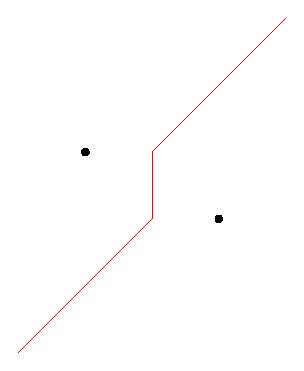
\includegraphics[scale=0.5]{3d/voronoi-cube-non-aligned}
    \hspace{2cm}
    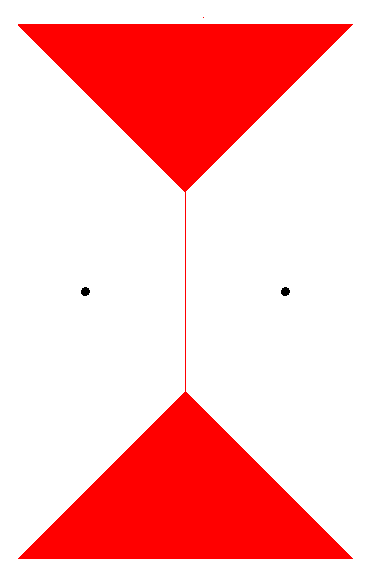
\includegraphics[scale=0.5]{3d/voronoi-cube-aligned}
    \caption{Bisector for the $ L^\infty $ norm: two non aligned points / two
        aligned points}
    \label{fig:3d-voronoi-cube}
\end{figure}

For computing the volume of $ \bigcup_{p \in P} B_N(p, r) $, we implemented two
different methods: a naive one and one based on inclusion-exclusion formula.  In
the naive one, we make the following approximation: instead of summing up over
all intersections $ V_N(p, P) \cap B_N(p, r) $, we sum up over all $ V(p, P)
\cap B_N(p, r) $. The influence of this choice under the functional we minimized
is described in Section \ref{sec:theory-3d-case}. We will see that the second
approached based on inclusion-exclusion formulae is also an approximated one.
There is also one method which is exact but we did not have the time to
implement it in our internship, it is based on 3D arrangements and overlays.

Firstly, we will define formally what we call a polyhedral norm. Then, we will
explain our naive method. Secondly, we will explain the inclusion-exclusion
formula we used in our second method. Then, we will talk about the choices we
made for the implementation and finally, we will run experiments to validate our
expectations.

% {{{1 POLYHEDRAL NORM
\section{Polyhedral norm}
\label{sec:polyhedral-norm}
A polyhedral norm is a function $ N $ defined as follows:

\begin{equation}
    \forall x \in \mathbb{R}^d,~ N(x) = \max_{i} (x | v_i)
\end{equation}
where the $ v_i $ are given vectors from $ \mathbb{R}^d $. This definition
implies that the unit ball for the norm $ N $ is a polyhedron. Indeed, if $ x
\in B_N(0, 1) $, then :

$$ N(x) \leq 1 \Longleftrightarrow \forall i,~(x | v_i) \leq 1 $$

So, the unit ball is defined by linear constraints. More precisely, it is an intersection
of half-spaces and so is a convex polyhedron $ K $. The vectors $ v_i $ are the
normal vectors to the facets of $ K $. We will denote by $ B_K(0, 1) $ the unit
ball defined by the convex polyhedron $ K $.

% {{{1 VOLUME OF A UNION OF POLYHEDRA
\section{Volume of a union of polyhedra}

In this section, we will show how to compute an approximation of the volume of
a union of polyhedra using two different methods: a naive one and one based on
inclusion-exclusion formula.

% {{{2 NAIVE METHOD
\subsection{Naive method}
We want to compute :

\begin{equation}
    Vol(\bigcup_{p \in P} B_N(p, r)) = \sum_p Vol(\bigcup_p B_N(p, r) \cap V(p, P))
\end{equation}

The idea of this method is to approximate $ Vol(\bigcup_p B_N(p, r) \cap V(p,
P)) $ by $ Vol(B_N(p, r) \cap V(p, P)) $. Then, we just have to compute the
intersection of half-spaces (see Section \ref{sec:3d-implementation} for
details). It is an approximation because, for example, if we want to compute the
perimeter of the boundary of squares in 2D, there is a difference between what
we want to compute and what we actually compute (see Figure
\ref{fig:3d-inclusion-exclusion-squares}): our computation is just an
approximation.

\begin{figure}[h]
    \centering

    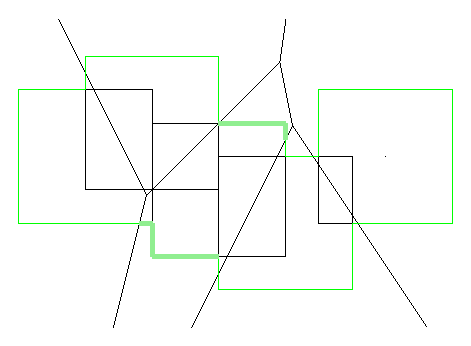
\includegraphics[scale=0.8]{3d/3d_perimeter_squares_truth}
    \hspace{2cm}
    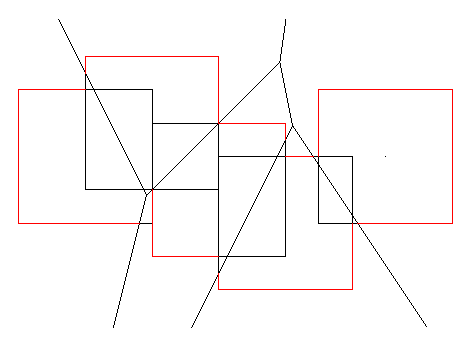
\includegraphics[scale=0.8]{3d/3d_perimeter_squares}
    \caption{In green, what we want and in red what we actually compute}
    \label{fig:3d-inclusion-exclusion-squares}
\end{figure}

% {{{2 INCLUSION-EXCLUSION FORMULA
\subsection{Inclusion-exclusion formula}

The inclusion-exclusion formula is a well-known formula which can be used to
compute the indicator function of a union of sets: given a finite number of sets
$ A = \{ A_1, \ldots, A_N \} $, we have:

\begin{equation}
    \indicator{\bigcup A_i} = \sum_{\emptyset \neq X \subseteq A} (-1)^{card X -
        1} \indicator{\bigcap X}
\end{equation}

This formula can also be expressed using the notion of nerve as shown in
\cite{attali2007inclusion}. We define the nerve of $ A = \{ A_x, x \in X \} $ to
be the simplicial complex \footnote{A simplicial complex is a generalization of
    a triangulation: it is a collection of simplices like vertices, edges,
    triangles, tetrahedra...} where a simplex $ \sigma $ exists between $ x_1
\ldots, x_k $ if $ \bigcap\limits_{i=1}^k A_{x_i} \neq \emptyset $. Then, we can
write the inclusion-exclusion formula as:

$$ \indicator{\bigcup A_x} = \sum_{\sigma \in Nerve(A)} (-1)^{\dim \sigma}
\indicator{\bigcap \sigma} $$
$ \sigma $ represents any simplex in the nerve. Its dimension is defined as: $
\dim \sigma = card \sigma - 1 $. If we consider a union of polyhedra, we can write a similar formula:

\begin{equation}
    \indicator{\bigcup B_N(p, r)} = \sum_{\sigma \in Nerve(\mathcal{B}_N)} (-1)^{\dim \sigma}
    \indicator{\bigcap \sigma}
    \label{eqn:incl_excl_simplices}
\end{equation}
where $ \mathcal{B}_N $ is the collection of all balls $ B_N(p, r), p \in P $.

Now, since the nerve can be a really big object, we want to restrict the
computation to what we call the $\alpha$-complex of a set of points:

\begin{definition} The $\alpha$-complex of a set of points $ X $ denoted by $
    Del(X, \alpha) $ is a subset of the Delaunay triangulation. To each simplex
    of the Delaunay triangulation, we can associate a characteristic
    radius: the radius of the smallest empty circle containing the simplex.

    Now, the $\alpha$-complex contains all the simplices of the Delaunay
    triangulation whose characteristic radius is smaller than $\alpha$.
\end{definition}

Now, we can ask if the formula \ref{eqn:incl_excl_simplices} is still valid if
we replace $ Nerve(\mathcal{B}_N) $ by $ Del(P, r) $.

If we want to prove this assertion, we may use the technique used to prove the
inclusion-exclusion formula for a union of balls. The proof starts by defining
the subcomplex $ L_p $ induced by a vertex $ p $.  We consider all the
polyhedrons that contains a given point $ x $ and we construct the nerve of it.
Formally, $ L_x = Nerve(\{ B_N(p, r),~x \in B_N(p, r)\}) $.

Then, when we evaluate the indicator function at $ x $ of the union, we can
decompose it in two parts: simplices of $ L_x $ and the other ones.

\begin{align*}
    \indicator{\bigcup B_N(p, r)}(x) &= \sum_{\sigma \in L_x} (-1)^{\dim \sigma}
    \indicator{\bigcap \sigma}(x) + \sum_{\sigma \notin L_x} (-1)^{\dim \sigma}
    \underbrace{\indicator{\bigcap \sigma}(x)}_{= 0 \text{ since } x \notin
        \sigma} \\
    &= \sum_{\sigma \in L_x} (-1)^{\dim \sigma} \\
    &= \chi(L_x)
\end{align*}

Here, $ \chi $ is the Euler characteristic.

Now, if we show that $ L_x $ is contractible (can be continuously deformed to a
point), we know that $ \chi(L_x) = 1 $. Obviously, we also have $
\indicator{\bigcup B_N(p, r)}(x) = 0 $ if $ x $ is not in the union and we will
conclude that the formula \ref{eqn:incl_excl_simplices} is true. But it appears
that there exists cases where the formula is not correct: see Figure
\ref{fig:incl_excl-examples}. In this figure, we can see that in the
$\alpha$-complex for the $ L^\infty $ norm, the triangle does not exist. It
means that in the formula the intersection between the three squares will not be
taken into account and so the final result will be incorrect. During this
internship, we did not have the time to estimate the error made by using this
formula.

\begin{figure}[h]
    \centering
    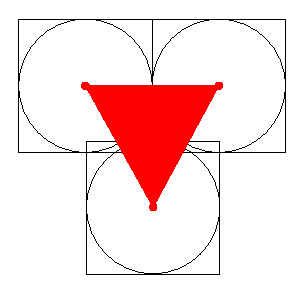
\includegraphics[scale=0.7]{3d/inclusion-exclusion-counter-l2}
    \hspace{2cm}
    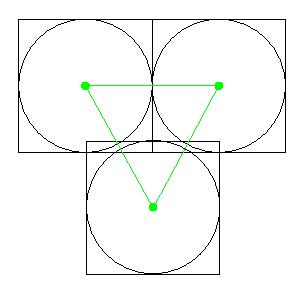
\includegraphics[scale=0.7]{3d/inclusion-exclusion-counter-linfty}
    \caption{Counter example where the formula is not correct, in red the
        $ L^2$ $\alpha$-complex and in green the $ L^\infty$ $\alpha$-complex.}
    \label{fig:incl_excl-examples}
\end{figure}

% {{{1 IMPLEMENTATION DETAILS
\section{Implementation details}
\label{sec:3d-implementation}

In this section, we will describe briefly how we implemented the two methods
previously described.

The libraries used are the same as the ones used in the 2D case except for the
rendering part: in 2D, we used a custom \texttt{QWidget} and in 3D, we choose to
use \texttt{QGLViewer}, an \texttt{OpenGL} based renderer.

\paragraph{Intersection computation}

For both methods, we need a way to compute intersection of half-spaces: for
the first one, we need to compute the intersection of a Voronoi cell and a
convex polyhedron and for the second one, we need to compute intersections of
convex polyhedra.

For the first method, the naive one, a Voronoi cell is represented implicitly as
a list of half-spaces (the planes defining the boundary of the cell).
Half-spaces are computed using the Delaunay triangulation. If we want to compute
the Voronoi cell of $ p $, we look at the neighbours in the Delaunay
triangulation of $ p $. Then, for every neighbour $ v $, the corresponding
half-space is the positive part of the bisector plane between $ p $ and $ v $.
The latter is the  plane passing through the midpoint of the segment $ [p, v] $
and whose normal vector is $ \vec{pv} $. Since the order of the traversal of the
vertices of the Delaunay triangulation is not, in general, the same as the
insertion one, we need to associate an index to a point (using a simple
\texttt{std::map}).

Then, a convex polyhedron $ K $ represents the unit ball for the polyhedral norm
$ N $ defined by $ K $. It is internally represented as a list of normal vectors
of each of its facets. Using this representation, one can compute the translated
polyhedron $ B_N(p, r) $ for a point $ p $ and a radius $ r $ by noticing that
it is the intersection of the half-spaces: $ \forall n,~ n_x x + n_y y + n_z z -
(p | n) - r \leq 0 $ where $ n $ is a normal vector of a facet.

In order to construct this intersection, we used the duality which allows us to
replace the computation of the intersection by the computation of the convex
hull (see \cite{preparata1979finding}) of the dual points: at each half-space, we
can associate a dual point and conversely.

Programmatically, we compute this intersection in the following manner:
\begin{enumerate}
    \item Compute the dual points while remembering which point is associated to
        which plane.
    \item Compute the convex hull of these dual points, it gives us a dual
        polyhedron. To each vertex, we associate the corresponding primal plane.
    \item To compute the primal polyhedron:
        \begin{enumerate}
            \item We first compute the primal vertices which are the dual of the
                dual facets: each dual facet has at least 3 vertices. We know
                the corresponding primal planes for these vertices.  Then, the
                corresponding primal vertex is the intersection of these 3
                planes.
            \item Secondly, the primal facets are constructed by circulating
                around the dual vertices. Each time there is an edge between two
                dual vertices, there is an edge between the two corresponding
                primal ones.
        \end{enumerate}
\end{enumerate}

See Appendix \appendixref{appendix:code-intersection} for a simplified version
of this algorithm:

For the second method, we also need a way to compute the $\alpha$-complex of a
set of points. This can be done using the \texttt{Alpha\_shapes\_3} package of
\texttt{CGAL} and the associated classification methods.

\paragraph{Automatic Differentiation integration}

Let's now explain in more details the integration of the automatic
differentiation tool. \texttt{CGAL} has the particularity to make easy for the
programmer to change the number type by using the concept of a \emph{Kernel}. A
\emph{Kernel} is a class that describes how numbers are stored in memory, how we
can construct things (like points, planes, bisectors...) and how to evaluate
predicates on objects (collinearity test, coplanarity test...).

There are multiple predefined kernels but we will quickly talk about two
particular ones. \texttt{Simple\_cartesian<NT>} is the most basic one: a number
will just be represented by \texttt{NT} and so it has inexact predicates
evaluation and inexact constructions.

\texttt{Exact\_predicates\_inexact\_constructions\_kernel} (in short
\texttt{Epick}) is a Kernel which use a technique called \emph{filtering} to
ensure the predicates are always evaluated in an exact manner. In short, the
predicate is first evaluated in an inexact way using interval arithmetic.  Then,
if the predicate, for example, has to check whether a value is zero or not then,
using interval arithmetic, it will need to check whether the resulting interval
contains zero or not. If this interval does not contains zero, then a decision
can be made. Otherwise, the computation is redone but this time using exact
arithmetic which, in all cases, will return an answer.

For the automatic differentiation, we replaced the \texttt{NT} type with our
custom class \texttt{AD}. \texttt{AD} is a class with two members: a value and a
vector of derivatives. It overloads all the classical arithmetic operations and
some mathematical functions (\texttt{sqrt}, \texttt{atan2}...). For example, the
implementation of \texttt{sqrt} for AD looks like this:
\lstinputlisting[language=C++]{code/sqrt_AD.h}

Then, for interfacing \texttt{AD} with \texttt{CGAL}, we choose the
\texttt{Simple\_cartesian<AD>} kernel. The choice of \texttt{Simple\_cartesian}
may seem inappropriate because the constructions are inexact but it is enough
for our applications.

% TODO

% {{{1 EXPERIMENTS
\section{Experiments}

% TODO

We compare the two different methods using various polyhedrons as base and
various point clouds.

We can choose for the polyhedron a sufficiently discretized sphere. We expect
the result to be the same as in the 2D case: gradients oriented like the outward
normal with a norm proportional to the mean curvature.

The figures \ref{fig:3d-mean-curvature-sphere-cube} give an example where the
point cloud is a sphere and the polyhedron is a cube.

\begin{figure}[h]
    \centering
    \begin{minipage}{0.32\linewidth}
        \centering
        \includegraphics[scale=0.35]{3d/sphere-polyhedron-200}
        \subcaption{Discretized sphere with 200 planes}
    \end{minipage}
    \begin{minipage}{0.32\linewidth}
        \centering
        \includegraphics[scale=0.3]{3d/sphere-1000}
        \subcaption{Initial point cloud: 1000 points on a sphere}
    \end{minipage}
    \begin{minipage}{0.32\linewidth}
        \centering
        \includegraphics[scale=0.3]{3d/sphere-sphere-1000-05}
        \subcaption{Gradients of the volume}
    \end{minipage}
    \caption{Sphere / cube}
    \label{fig:3d-mean-curvature-sphere-cube}
\end{figure}

We remark that the gradients are oriented like the outward normals and that
norms of these gradients seem relatively constant. This confirms the fact that
we can simulate our work in 2D (mean curvature flow) by choosing a sufficiently
discretized sphere.

We also did some experiments for checking the convergence of the flow. Figures
\ref{fig:3d-flow-sphere-cube} and \ref{fig:3d-flow-sphere-bipyramid} give
examples where the point cloud is a sphere and the polyhedron is a cube and a
bipyramid. On these examples, we can see that the flow seems to converge towards
the polyhedron we choose.

\begin{figure}[h]
    \centering
    \begin{minipage}{0.32\linewidth}
        \centering
        \includegraphics[scale=0.4]{3d/sphere-cube-0}
        \subcaption{Initial sphere with 1000 points}
    \end{minipage}
    \begin{minipage}{0.32\linewidth}
        \centering
        \includegraphics[scale=0.4]{3d/sphere-cube-10}
        \subcaption{After 10 iterations}
    \end{minipage}
    \begin{minipage}{0.32\linewidth}
        \centering
        \includegraphics[scale=0.3]{3d/sphere-cube-cube}
        \subcaption{Shape of the cube}
    \end{minipage}

    \caption{Flow of a sphere under a cube}
    \label{fig:3d-flow-sphere-cube}
\end{figure}

\begin{figure}[h]
    \centering
    \begin{minipage}{0.32\linewidth}
        \centering
        \includegraphics[scale=0.4]{3d/sphere-cube-0}
        \subcaption{Initial sphere with 1000 points}
    \end{minipage}
    \begin{minipage}{0.32\linewidth}
        \centering
        \includegraphics[scale=0.4]{3d/sphere-bipyramid-10}
        \subcaption{After 10 iterations}
    \end{minipage}
    \begin{minipage}{0.32\linewidth}
        \centering
        \includegraphics[scale=0.3]{3d/sphere-bipyramid-bipyramid}
        \subcaption{Shape of the bipyramid}
    \end{minipage}

    \caption{Flow of a sphere under a bipyramid}
    \label{fig:3d-flow-sphere-bipyramid}
\end{figure}

\section{Conclusion}

In summary, we saw, in this chapter, another type of flow. We used the same
techniques as the ones developed in Chapter \ref{chapter:2d} by replacing a
union of balls with a union of convex polyhedra.

We saw that the obtained flow has different properties than the mean curvature
flow: the convergence shape will depend on which polyhedron we chose.

% TODO:

% TODO:
% - comparaison des différentes méthodes
% - résultats

% vim: set spelllang=en filetype=tex :

\chapter{Conclusion \& Perspectives}

% TODO:

% vim: set spelllang=en :


\backmatter
\appendix

% Appendix
\chapter{Automatic Differentiation}

The automatic differentiation is a technique used for computing the derivatives,
gradient of expressions. It is not the same as the symbolic or the numerical
differentiation.

Indeed, automatic differentiation can be used to compute derivatives of programs
and not only mathematical functions without using approximations like with
numerical differentiation.

Let us suppose that we want to compute the derivative of a function $ f $ with a
single one dimensional argument $ x $. To do that, we will replace the number
type that is to say that we will replace $ x $ by $ x + \epsilon x' $ where $
\epsilon $ with the property $ \epsilon^2 = 0 $. Then, we overload all the
arithmetical operations: addition, subtraction, multiplication, division.

Then we call $ f $ with this variable: $ f(x + \epsilon x') = y + \epsilon y'
$. We conclude that $ y = f(x) $ and $ y' = x' f'(x) $ . Indeed for small values
of $ \epsilon $, we have the first order Taylor expansion: $ f(x + \epsilon x') =
f(x) + \epsilon x' f'(x) + ... $. $ x' $ is called a seed and can be chosen
arbitrarily, we can for instance choose $ x ' = 1 $ and so $ y' = f'(x) $.

This process can be easily extended to handle functions like $ f : \R^n
\rightarrow \R $ in order to compute gradients of such functions. This is what
we did: we considered a function over $ n $ points as $ f : \R^{2n} \rightarrow
\R $.

This technique is interesting because it allows us to compute accurate
derivatives of functions very easily and efficiently. Indeed, we only have to
change the number type and write the good implementations of the basic
arithmetic operations.
In \texttt{CGAL}, this is easy to do since the library is already parametrized
by the number type.

% TODO

% vim: set spelllang=en :


% Bibliography
\bibliographystyle{plain}
\bibliography{bibfile}

\end{document}

